\subsection{MCMC Sampling with Neuronized Priors}

Under the linear regression model mentioned previously, the joint posterior distribution of the parameters follows the form of Equation \eqref{eq:post_joint}. Therefore, the full conditions can be written as follows. The conditional posterior distribution of $\bm{w}$. given other parameters is a Gaussian distribution,
\begin{equation} \label{eq:w_condi}
    \bm{w} | \bm{y}, \bm{\alpha}, \sigma^2, \tau_w^2 \sim N(\tilde{\mu}, \sigma^2 \tilde{\Sigma}),
\end{equation}
where $\tilde{\Sigma} = (D_\alpha X^T X D_\alpha + \sigma^2 \tau_w^{-2} I)^{-1}$, and $\tilde{\mu} = \tilde{\Sigma} D_\alpha X^T \bm{y}$, and $D_\alpha$ is defined as in Section \ref{sec:neu_def}. However, when the number of coefficients $p$ is large relative to the number of observations $n$, the computational complexity of solving $(D_\alpha X^T X D_\alpha + \sigma^2 \tau_w^{-2} I)^{-1}$ is highly expensive. \citet{shin2021neuronized} adopts the fast sampling procedure proposed in \citet{bhattacharya2016fast}, which reduces the complexity from $O(p^3)$ to $O(n^2p)$.

Because $w_j$ and $\alpha_j$ are highly correlated a posteriori, the algorithm draw samples from the posterior through the following scheme. For $j=1,\dots, p$, we draw sample $\alpha_j$ conditional on $\bm{\alpha}_{-j}$ and $\bm{w}$, that is, $\alpha_j^* \sim \pi(\alpha_j| \bm{y}, \bm{w}_{-j}, \bm{\alpha}_{-j})$ by a RWMH algorithm, based on the log-target function,
\begin{equation} \label{eq:log-target}
    - \log (v_j) / 2 - \alpha_j^2 /2 + v_j m_j^2 / (2\sigma^2),
\end{equation}
where $v_j = X^T_j X_j T(\alpha_j - \alpha_0) + \sigma^2 / \tau_w^2$, and $m_j = \vr^T X_j T(\alpha_j - \alpha_0)/v_j$. And then sample $w_j$ from $\pi(w_j| \bm{y}, \bm{\alpha_j}, \alpha_j^*)$, conditional on other parameters. 
\begin{equation} \label{eq:w_j_sample}
    w_j | \vy, \valpha_{-j},\alpha_j, \vw_{-j}, \sigma^2, \tau_w^2 \sim N(m_j, \sigma^2 v_j^{-1})
\end{equation} 
%Here $N(\alpha_j^{(t)}, 2^2)$ is used as the proposal distribution. 
For continuous neuronized priors, $\alpha_0$ is set to be 0 and for neuronized SpSL, a hyper parameter is imposed on $\alpha_0$ which is discussed in the next section. We implemented this algorithm with the help of the NPrior package included in \citet{shin2021neuronized}, and conducted simulation and real data examples in later sections. The detailed algorithm is shown in Algorithm \ref{alg:neu_MCMC}.

\begin{algorithm}[H]
\caption{A general MCMC algorithm for neuronized priors} \label{alg:neu_MCMC}
\begin{algorithmic}
\Require Initialization of $\valpha,\alpha_0, \vw, \sigma^2$.
\State Sample $\vw$ conditional on $\vy, \valpha, \sigma^2$ from Equation \eqref{eq:w_condi}.
\For {$i = 1,\dots, N$}
\State Set $\vr = \vy - X\vtheta(\valpha,\vw)$.
\For {$j = 1,\dots, p$}
\State Update $\vr = \vr + X_jT(\alpha_j-\alpha_0) w_j$.
\For {$irep=1,\dots,N$}
\State Sample $\alpha_j$ from $\alpha_j | \vy, \valpha_{-j}, \vw_{-j} ,\sigma^2, \tau_w^2$ using a RWMH step with Equation \eqref{eq:log-target}.
\State Sample $w_j$ from $w_j | \vy, \valpha_{-j},\alpha_j, \vw_{-j}, \sigma^2, \tau_w^2 $ with Equation \eqref{eq:w_j_sample}.
\EndFor
\State Update $\vr = \vr - X_jT(\alpha_j-\alpha_0) w_j$.
\EndFor
\State Sample $\sigma^2$ from $\sigma^2 | \vy, \valpha, \vw, \tau_w^2$.
\State Sample $\delta$ based on the method described in Section \ref{sec:samp_alpha0}.
\EndFor
\end{algorithmic}
\end{algorithm}

\subsection{Sample $\alpha_0$ efficiently} \label{sec:samp_alpha0}

Because of the high correlation between $\alpha_0$ and the $\alpha_j$’s, a naive MH approach in which $\alpha_0$ is updated by a MH step conditioned on $\valpha$ is highly inefficient. Therefore, \citet{shin2021neuronized} adopts a group-move via the generalized Gibbs sampling formulation proposed in \cite{liu2000generalised} which updates $\valpha$ and $\alpha_0$ simultaneously by a common shift $\delta \in \mathbb{R}$. Specifically, $(\valpha,\alpha_0)$ is updated in the way that
$$ (\valpha, \alpha_0) \rightarrow (\valpha + \delta \bm{1}, \alpha_0 + \delta),$$
where $\delta$ is sampled from $g(\delta) \propto \pi^*(\valpha + \delta \bm{1}, \alpha_0 + \delta)$, and $\pi^*(\valpha, \alpha_0)$ is the conditional posterior density for $\valpha$ and $\alpha_0$. 

When $a_0 = b_0 = 1$ in the prior, $g(\delta) = N((\valpha^T\valpha + \alpha_0)/(p+1) , (p+1)^{-1})$. Otherwise, an extra approximation step is needed. The algorithm in \citep{shin2021neuronized} uses a multiple-try MH independence sampler (MTM-IS) to sample $\delta$. It proposes multiple candidates $\delta_i$'s drawn independently from a proposal distribution and then chooses one from them with probability proportional to their importance weights.

\subsection{Computational advantage of neuronized discrete SpSL} \label{sec:neu_dis_spsl_com}

The paper \citep{shin2021neuronized} shows that a fully collapsed and a half collapsed Gibbs sampler can be applied to efficiently sample from the posterior with the standard discrete SpSL priors. However, both of the methods are mot feasible when the continuous parameters cannot be analytically integrate out. It demonstrates that the neuronized priors are computationally efficient while achieving the same effect as the standard discrete SpSL priors, even if the marginals cannot be derived analytically. As is shown in the proposition in the paper, with a ReLU activation function in the neuronized prior, the conditional distribution $\pi(\alpha_j|\vy, \vw_{(-j)}, \valpha_{(-j)})$ is a mixture of two truncated Gaussians and therefore can be sampled exactly.

Another advantage of using the ReLU activation function is that when sampling $\vw$, the conditional posterior distribution can be decomposed as a product of independent Gaussian densities so that the numerical inversion of matrix to compute $\tilde{\Sigma}$ in Equation \eqref{eq:w_condi} can be avoided.

\subsection{A Scalable Algorithm for Finding Posterior Modes}

For large dataset, the computation of MCMC algorithm may not be practical so that we may consider optimization-based algorithms. Several optimization methods have been proposed to conduct the posterior inference with the SpSL priors. For example, EMVS \citep{rovckova2014emvs} and SSLASSO \citep{rovckova2018spike} are two optimization procedures for the Bayesian SpSL variable selection problem.

\citet{shin2021neuronized} proposes a coordinate-ascent algorithm for neuronized (CAAN) priors which finds the MAP estimator. To reduce the chance of being trapped in a local optimum, CAAN uses a warm start strategy by initializing the hyper-parameter leading to a weak shrinkage and increasing the strength of shrinkage gradually. 

The algorithm uses a temperature scheme with temperatures $t_k$ such that $t_0 \leq \cdots \leq t_{2L+1}$. At each temperature $t_k$, the coordinate ascent iterations are conducted $M$ times. The CAAN algorithm updates the value of $\alpha_j$ by optimizing it when fixing other parameters $\bm{\alpha}_{-j}$ and $\bm{w}$. This optimization is easily feasible because the log posterior with respect to $\alpha_j$ is a simple linear combination of a quadratic function and a function of $T(\alpha_j-\alpha_0)$. And $\bm{w}$ is updated taking the advantage of conjugacy. To get rid of trapping in a local optima, a random noise $\xi \sim \exp (1)$ is added in the first $L$ levels of temperature scheme. By default, we set $M=20$, $L=10$, $N=20$, $t_k = (3-2k/L)^2$ for $k= 1, \dots L$, and $ t_{L+1} = \cdots = t_{2L}$. Detailed algorithm is provided in Algorithm \ref{alg:caan} . We implemented this algorithm and conducted simulation studies using it in later sections.

\begin{algorithm}[H]
\caption{The coordinate-ascent algorithm for neuronized prior (CAAN)} \label{alg:caan}
\begin{algorithmic}
\Require Initialization of $\valpha,\alpha_0, \vw, \sigma^2$.
\State Set a candidate set of temperature, $\{t_{(1)}, \dots, t_{(2L+1)}\}$.
\For {$l = 1,\dots, 2L+1$}
\State Set $t = t_{(l)}$.
\State Set $\vr = \vy - X\vtheta(\valpha,\vw)$.
\For {$irep=1,\dots,M$}
\For {$j = 1,\dots, p$}
\State Update $\vr = \vr + X_j T(\alpha_j - \alpha_0)w_j$.
\State Update $\alpha_j$ by optimizing the log marginalized posterior in Equation \eqref{eq:log-target} with respect to $\alpha_j$.
\State Update $w_j$ from $w_j | \vy, \valpha_{-j},\alpha_j, \vw_{-j}, \sigma^2, \tau_w^2 $ with Equation \eqref{eq:w_j_sample}.
\State Update $\vr = \vr - X_jT(\alpha_j-\alpha_0) w_j$.
\EndFor
\State Every $N$ iterations,
\State  Update $\sigma^2 = (\normtwo{\vy-X\vtheta(\valpha,\vw)}^2/t + 2b_1)/\{n+2a_1+2\}$.
\If{$l \leq L$}
    \State Set $\sigma^2 = \sigma^2 + \xi$, where $\xi \sim \exp(1)$.
\EndIf
\State  Update $\alpha_0 = \{\sum_{j=1}^p 1(\alpha_j > \alpha_0) + a_0 -1\}/ (p+b_0 -2).$
\EndFor
\EndFor
\end{algorithmic}
\end{algorithm}


\subsection{Comparison With Other Posterior Optimization Procedures}

We conduct simulation to compare the performance of the proposed CAAN and other optimization methods finding the MAP, parallel to what the paper did. We evaluate the property of the CAAN algorithm \citep{shin2021neuronized} and the EMVS \citep{rovckova2014emvs}, which evaluates the MAP estimator Based on an EM formulation. Two metrics are investigated in the study, the mean-squared error (MSE) and the extended Bayesian information criterion (EBIC), which is, 
$$ \text{EBIC} = \text{BIC} + \zeta |\bm{k}| \log p,$$
where $\bm{k}$ is the set of selected variables, $\zeta$ is a tuning parameter (here, $\zeta = 1$), and BIC is the Bayesian information criterion.

We generate synthetic data by setting the error variance $\sigma^2 = 1$, and the first 10 elements in the coefficient vector to be randomly 2 or -2, and the rest 0. For EBIC, we use $\nu_1 = 100$ and $\nu_0^{-1}$ takes value from $(1,1000)$. Values of EBIC and log-MSE are evaluated as iteration increases.

Figure \ref{fig:Opt_comparison} shows the optimization paths of EMVS and CAAN. We can see from the results that the optimization paths of EMVS quickly converged to some sub-optimal models, corresponding to different solutions when started with different random initializations. Although both procedures failed to provide consistent results when initialized with different starting configurations, CAAN was more stable than EMVS.

\begin{figure}[tp]
     \centering
     \begin{subfigure}[b]{0.45\textwidth}
         \centering
         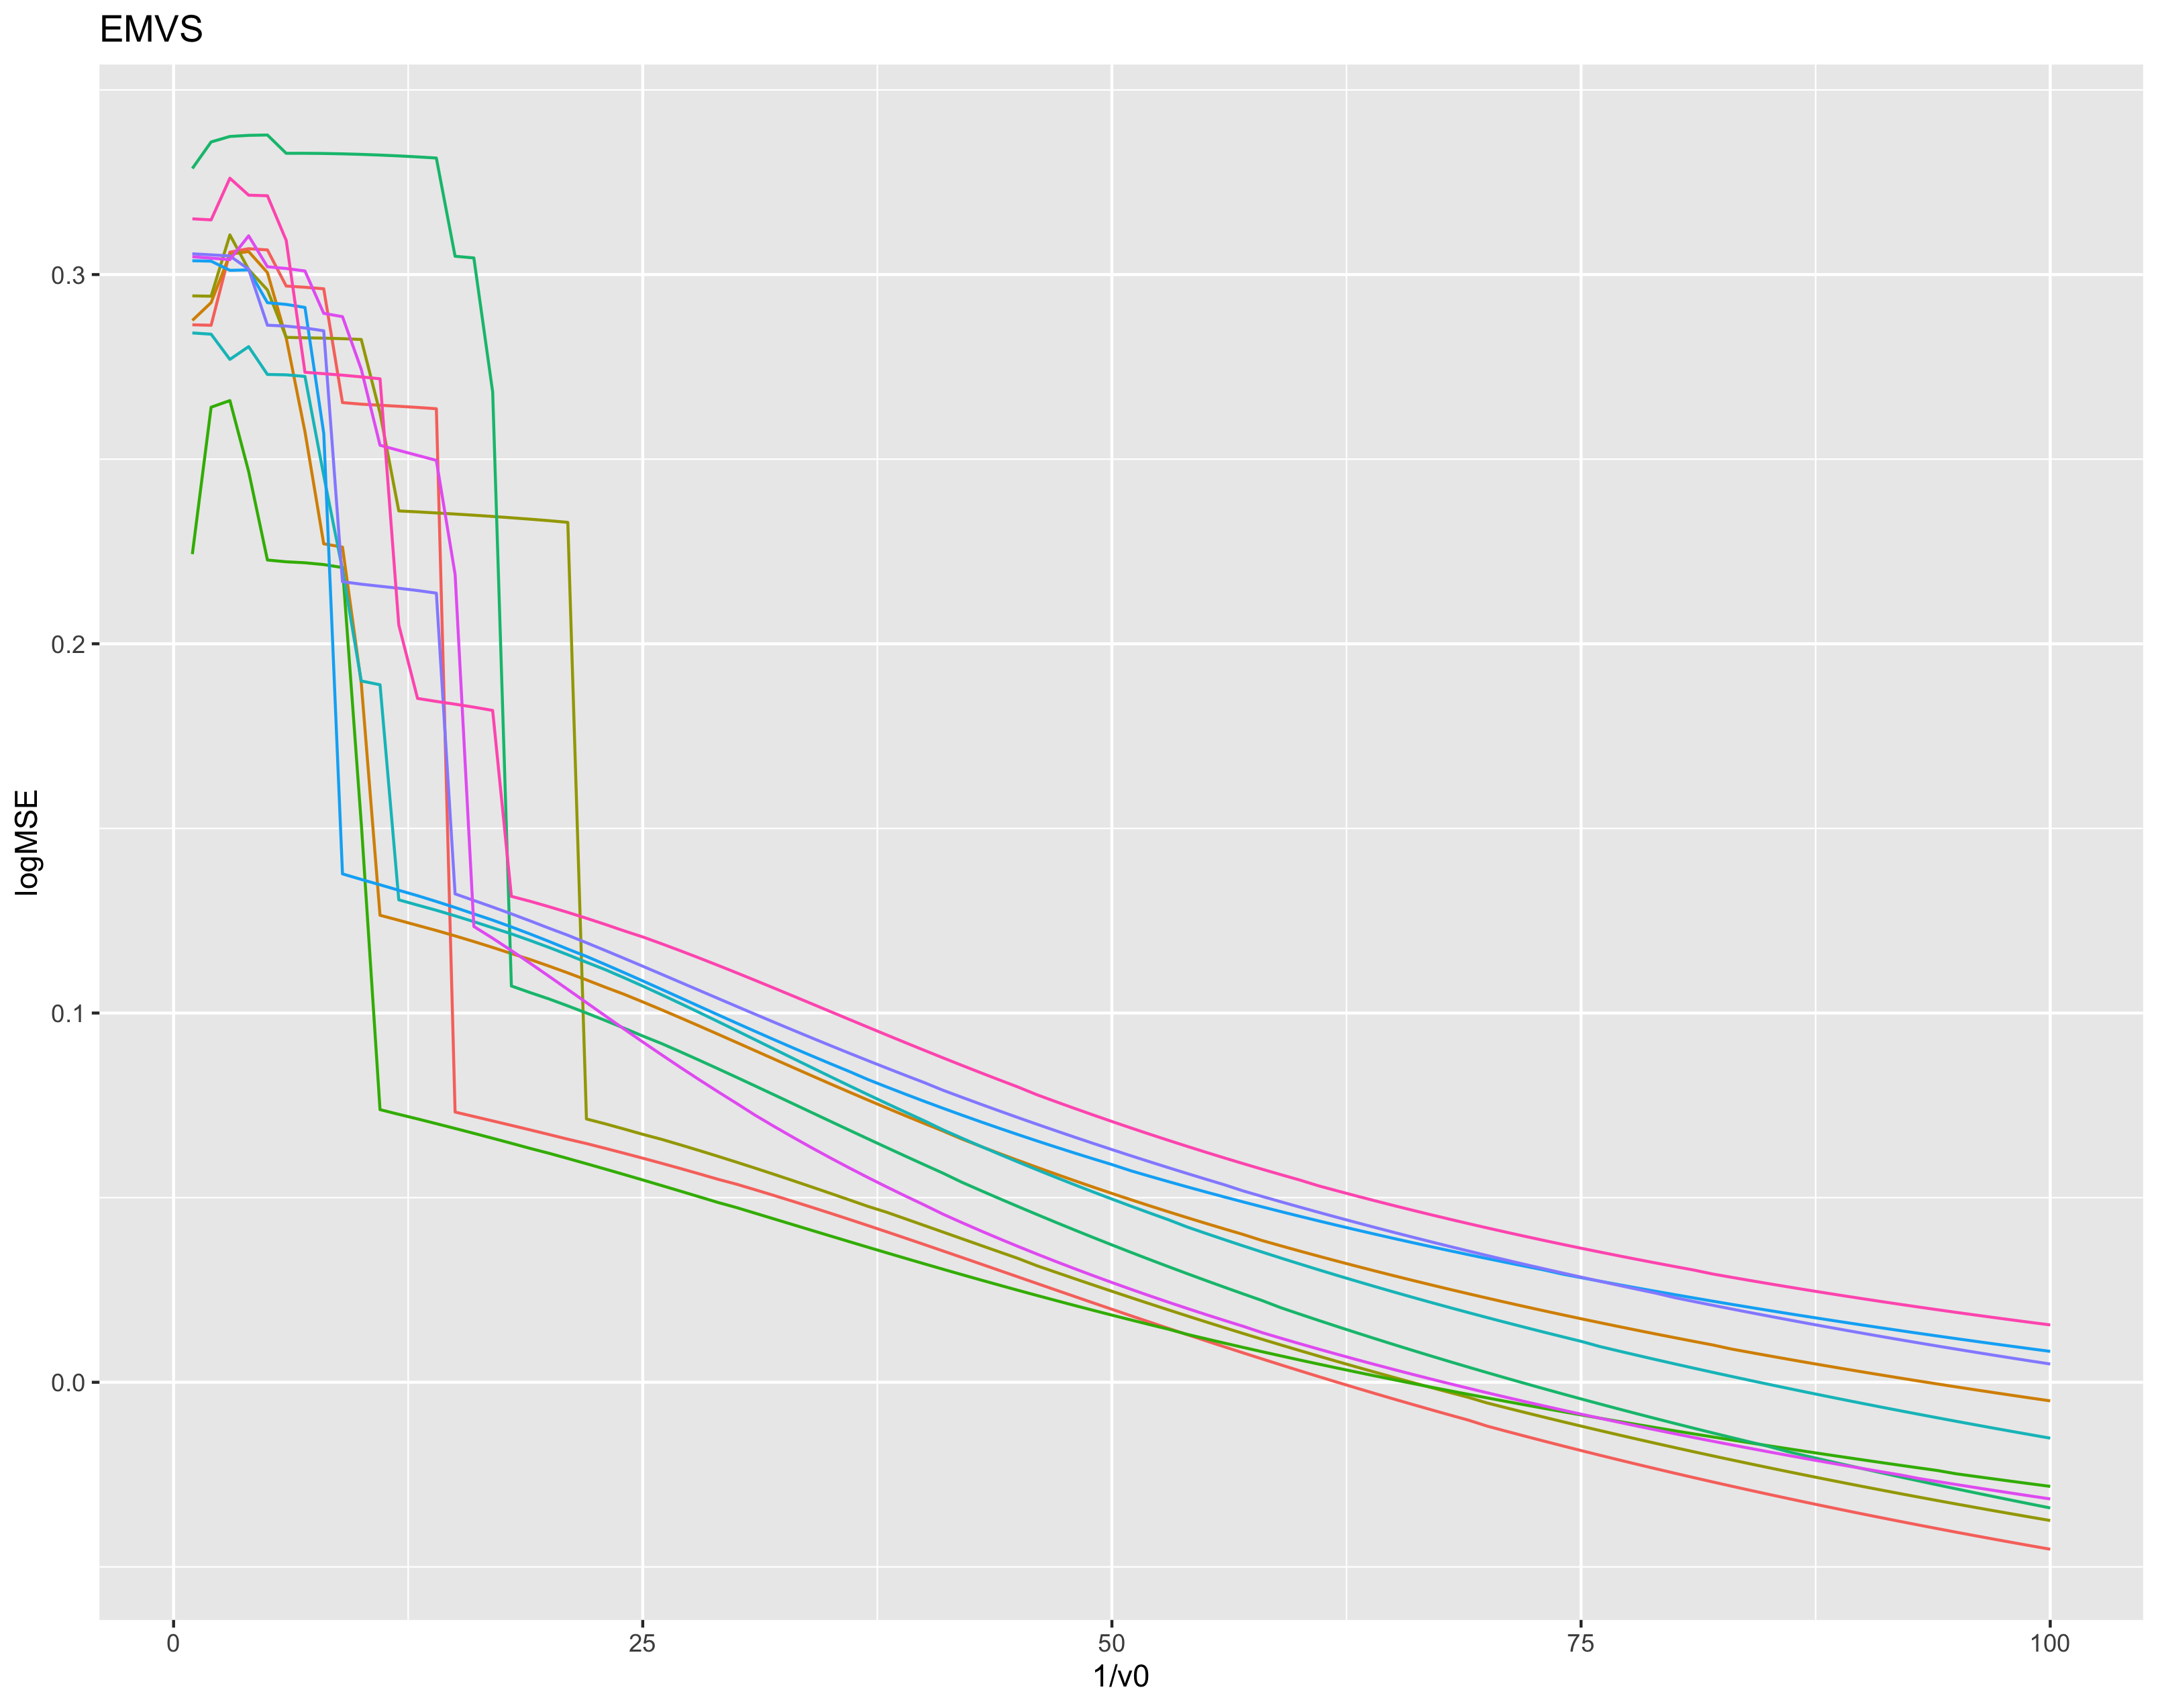
\includegraphics[width=\textwidth]{Figures/EMVS_MSE.png}
     \end{subfigure}
     \hfill
     \begin{subfigure}[b]{0.45\textwidth}
         \centering
         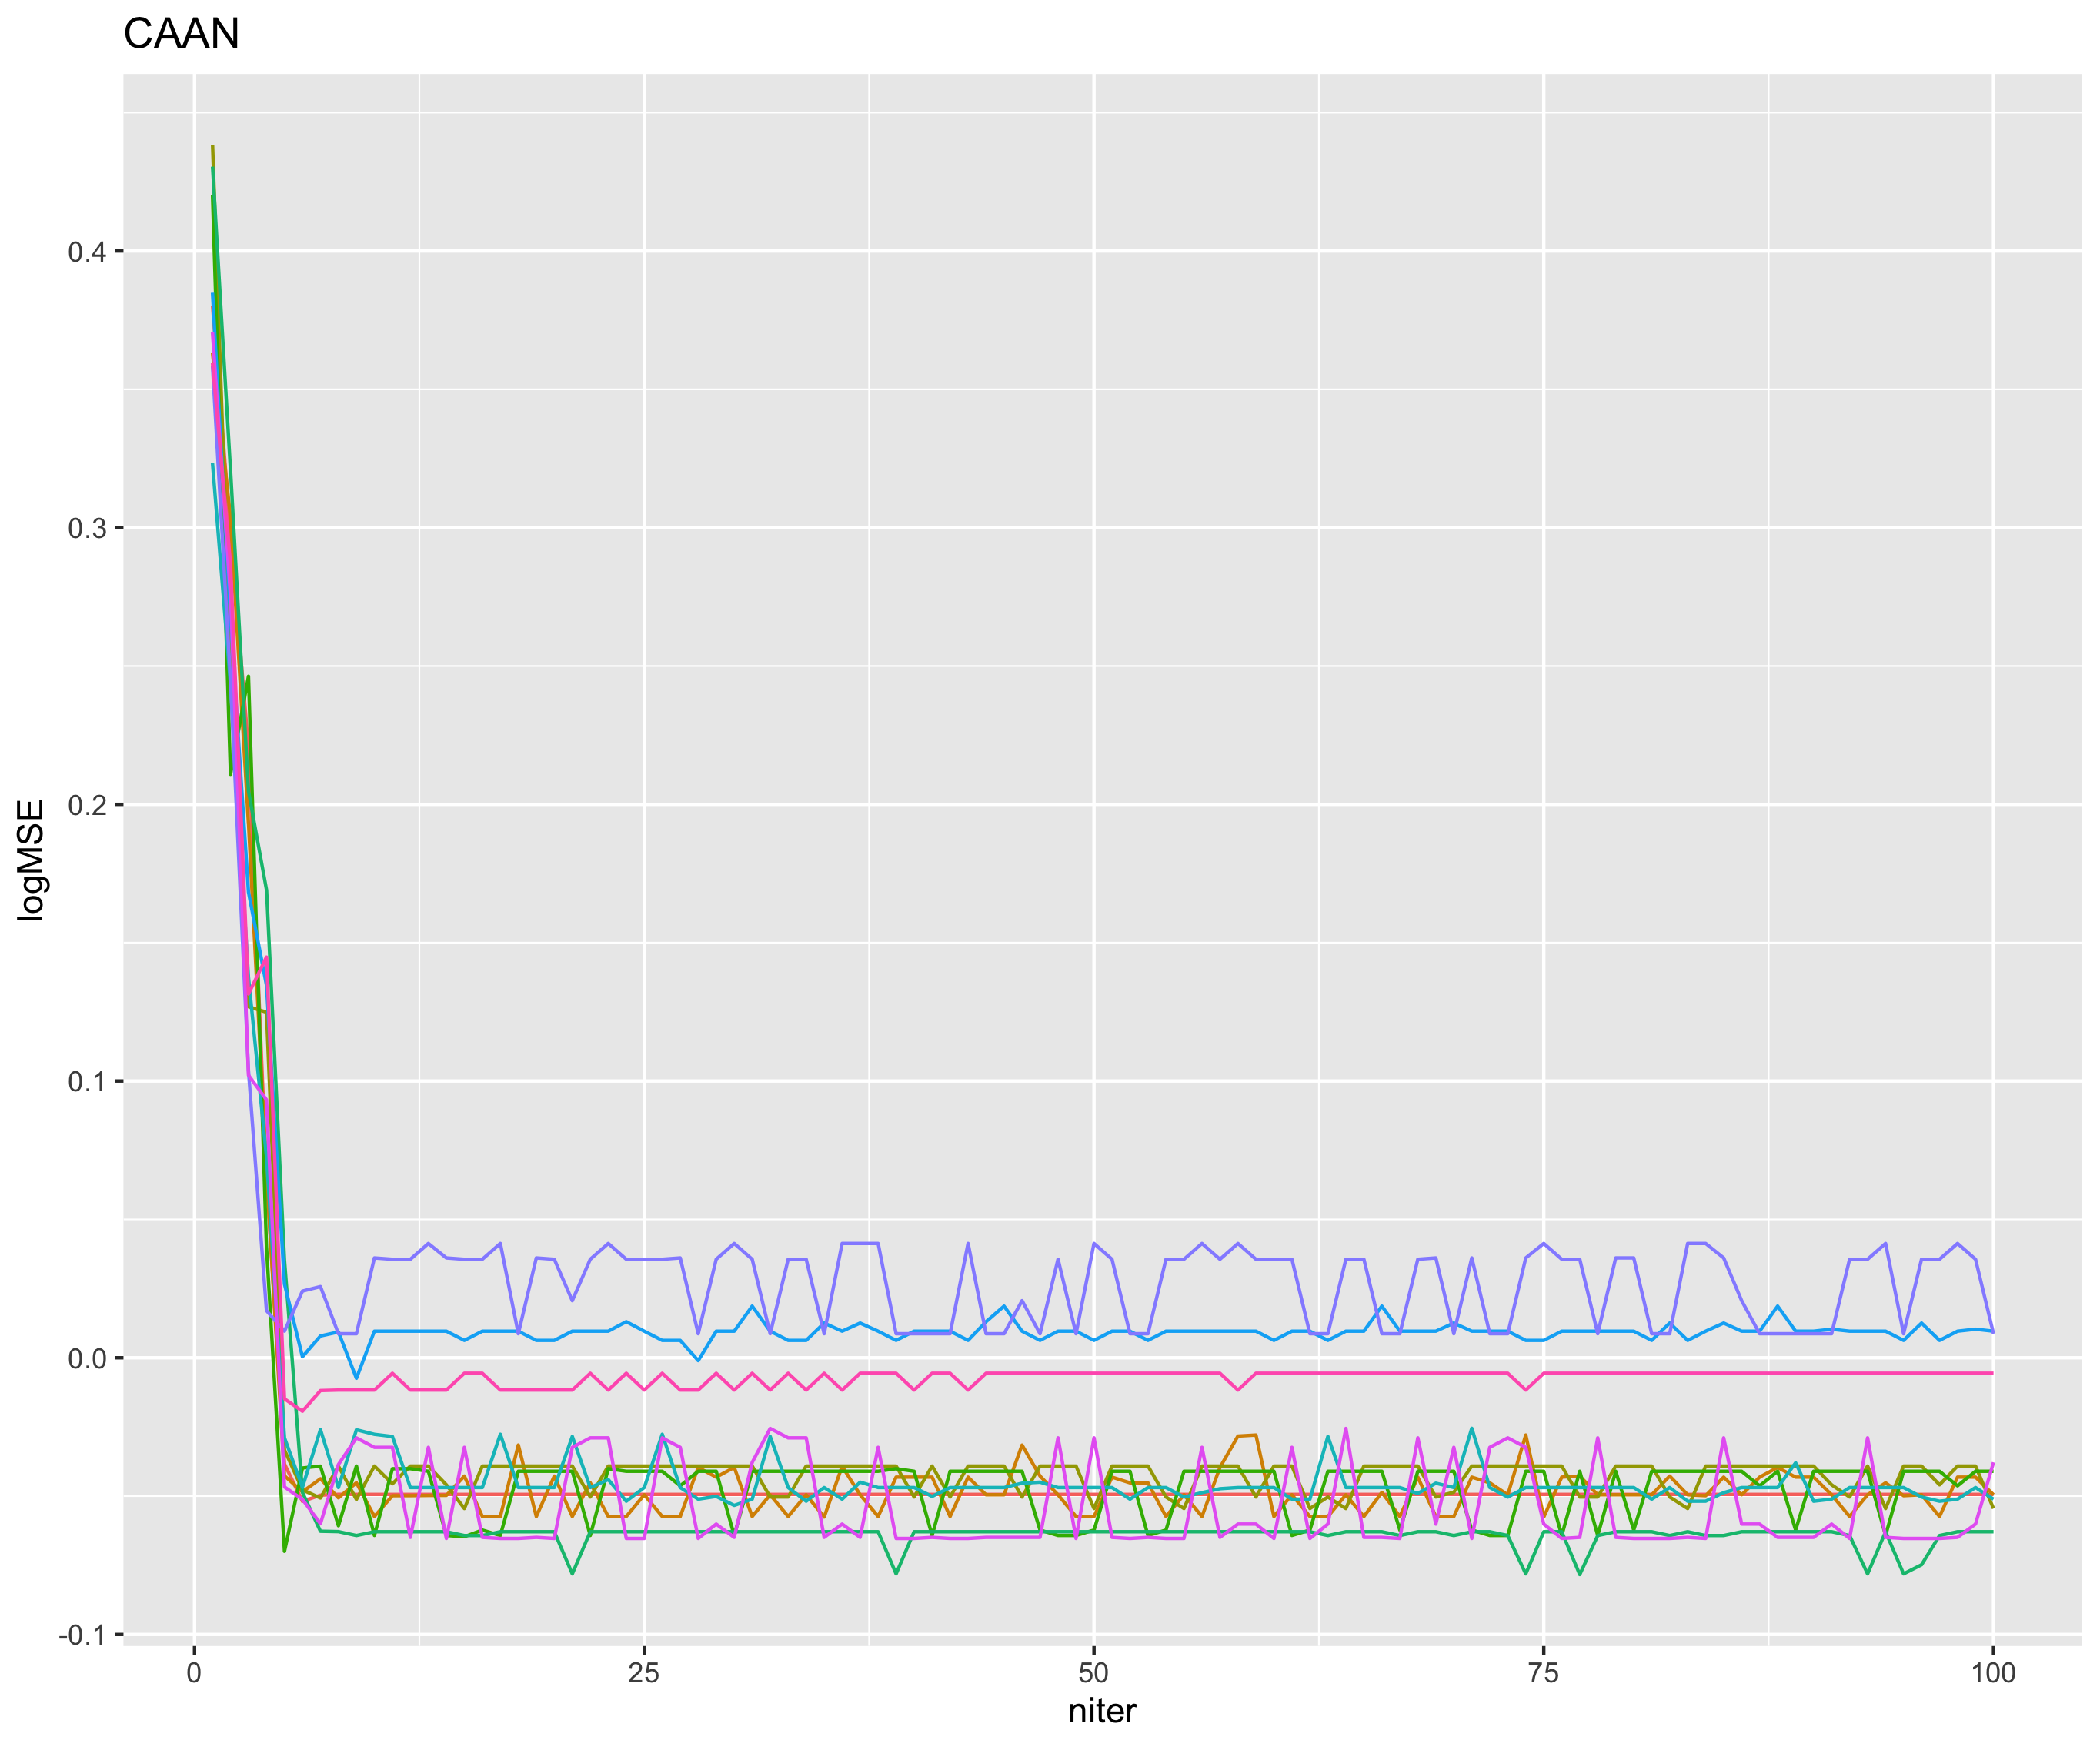
\includegraphics[width=\textwidth]{Figures/CAAN_MSE.png}
     \end{subfigure}
     \hfill
     \begin{subfigure}[b]{0.45\textwidth}
         \centering
         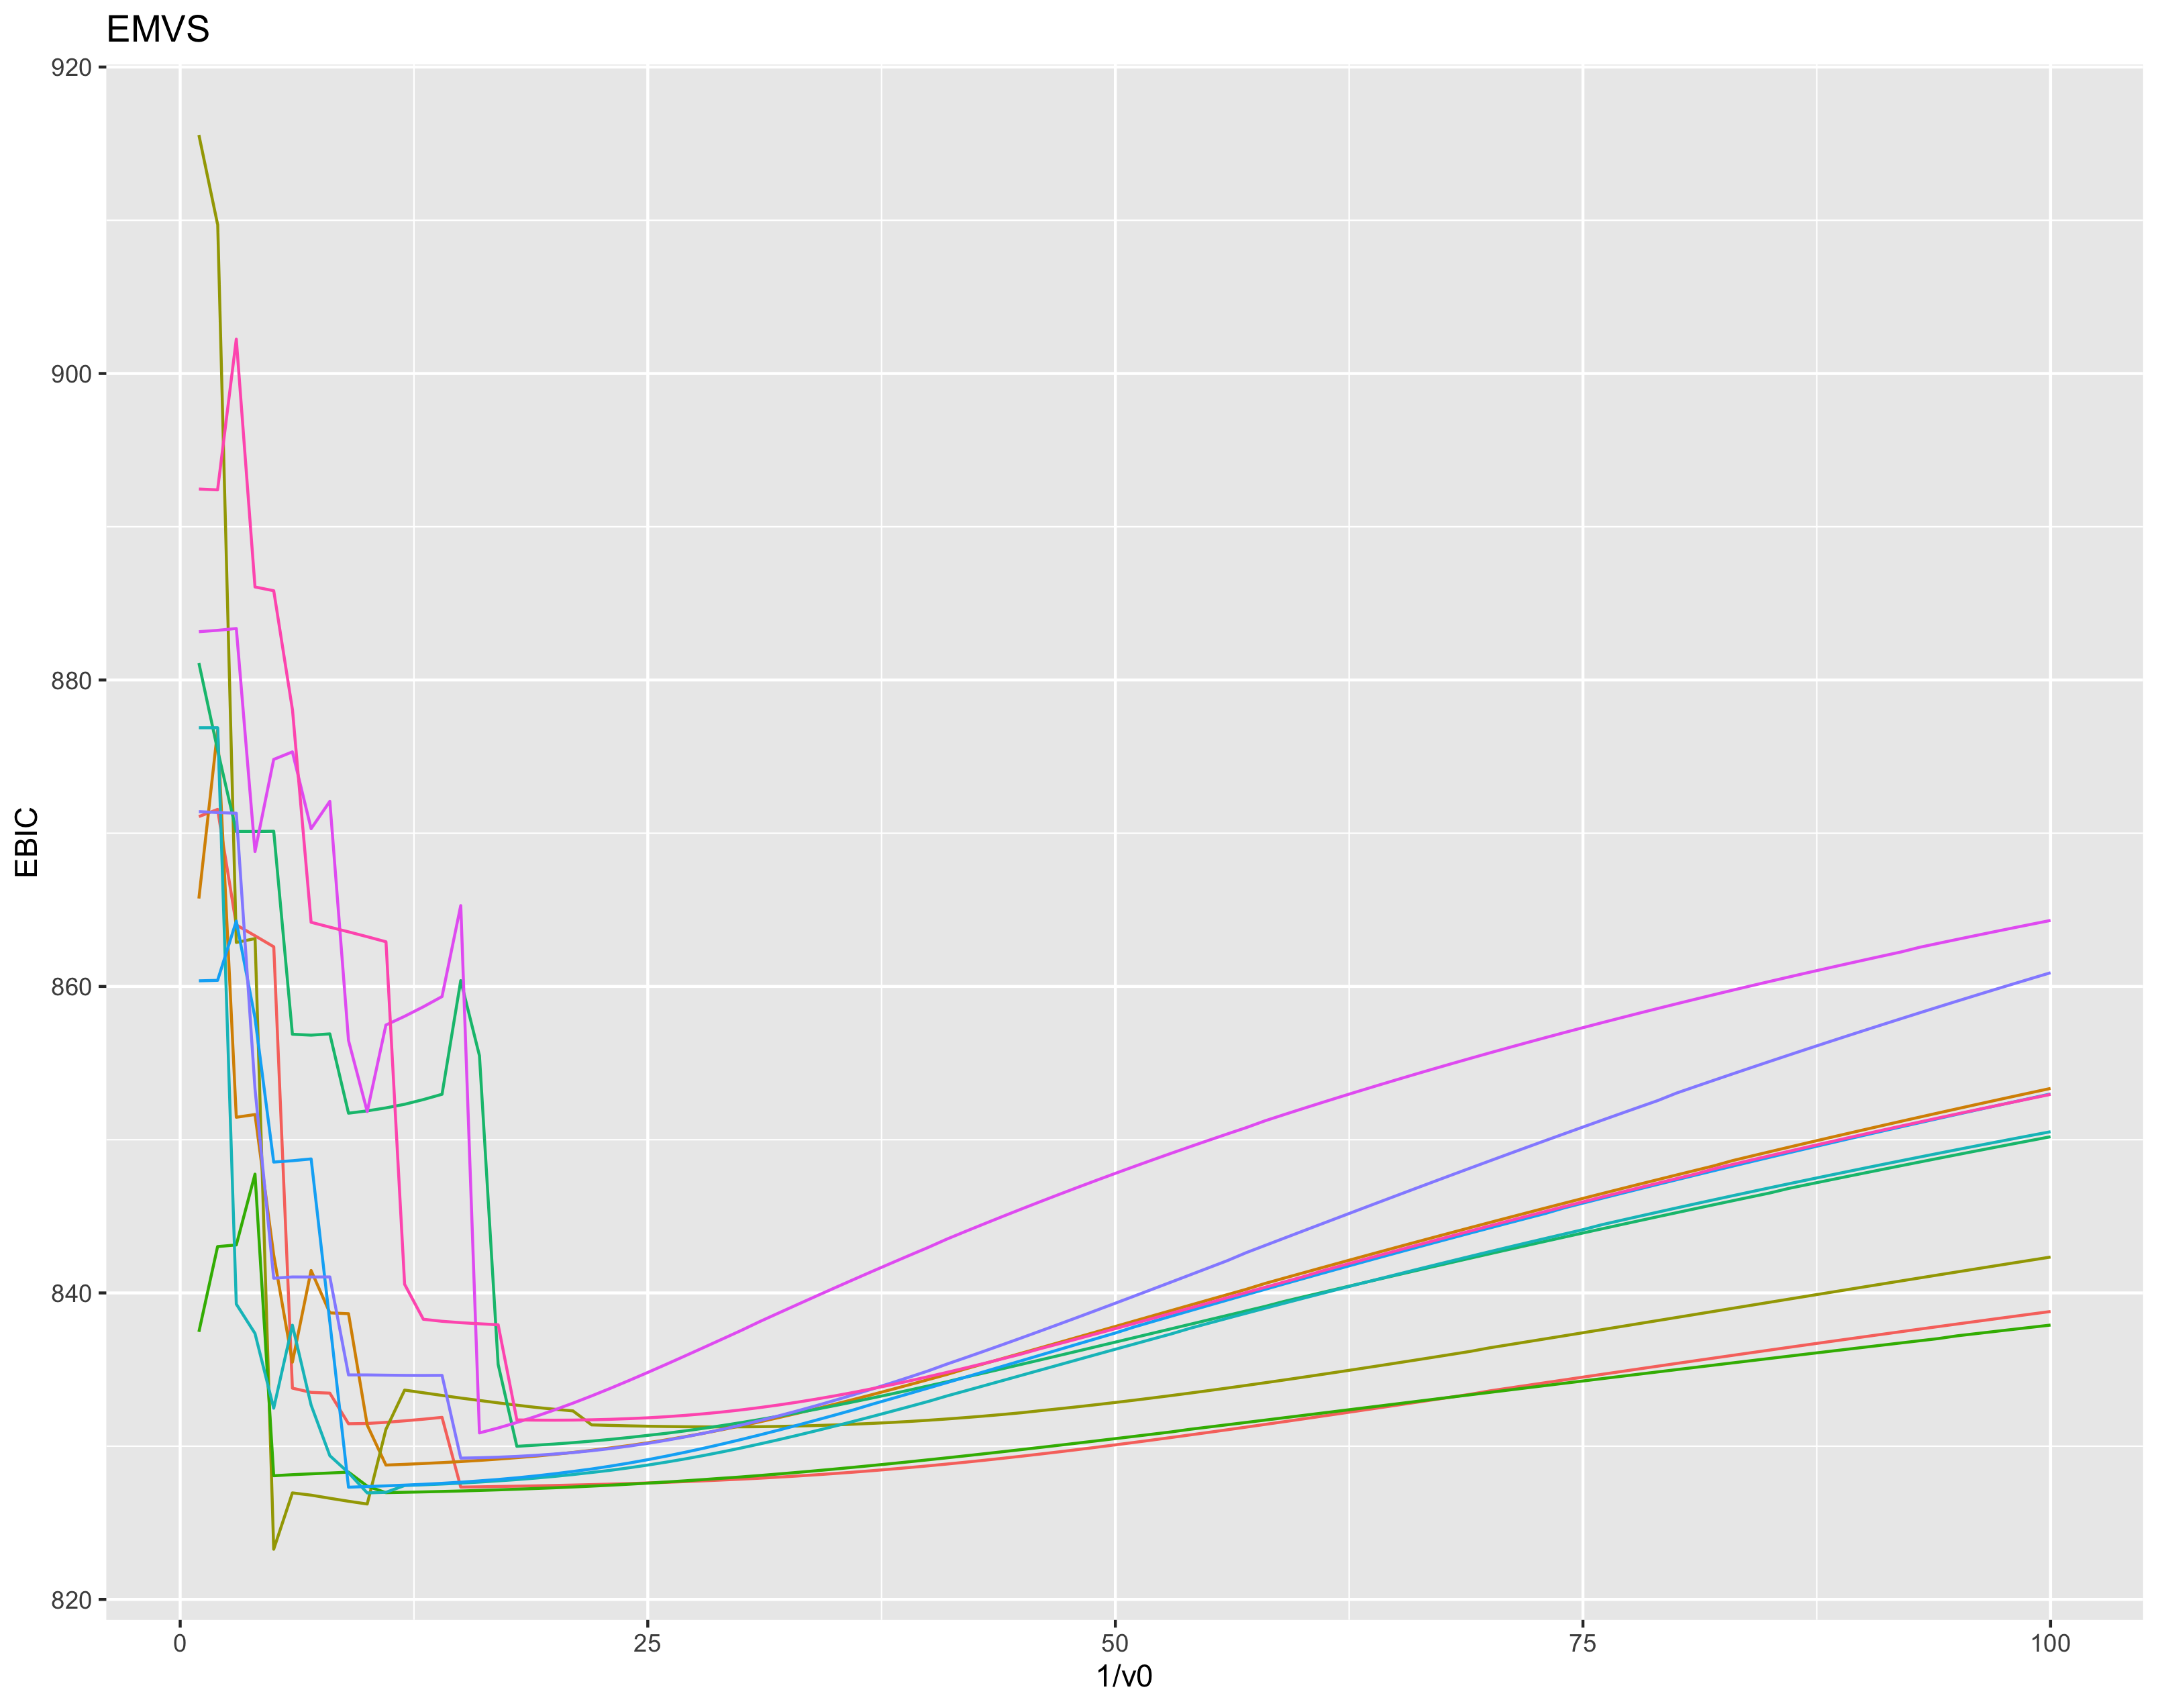
\includegraphics[width=\textwidth]{Figures/EMVS_EBIC.png}
     \end{subfigure}
     \hfill
     \begin{subfigure}[b]{0.45\textwidth}
         \centering
         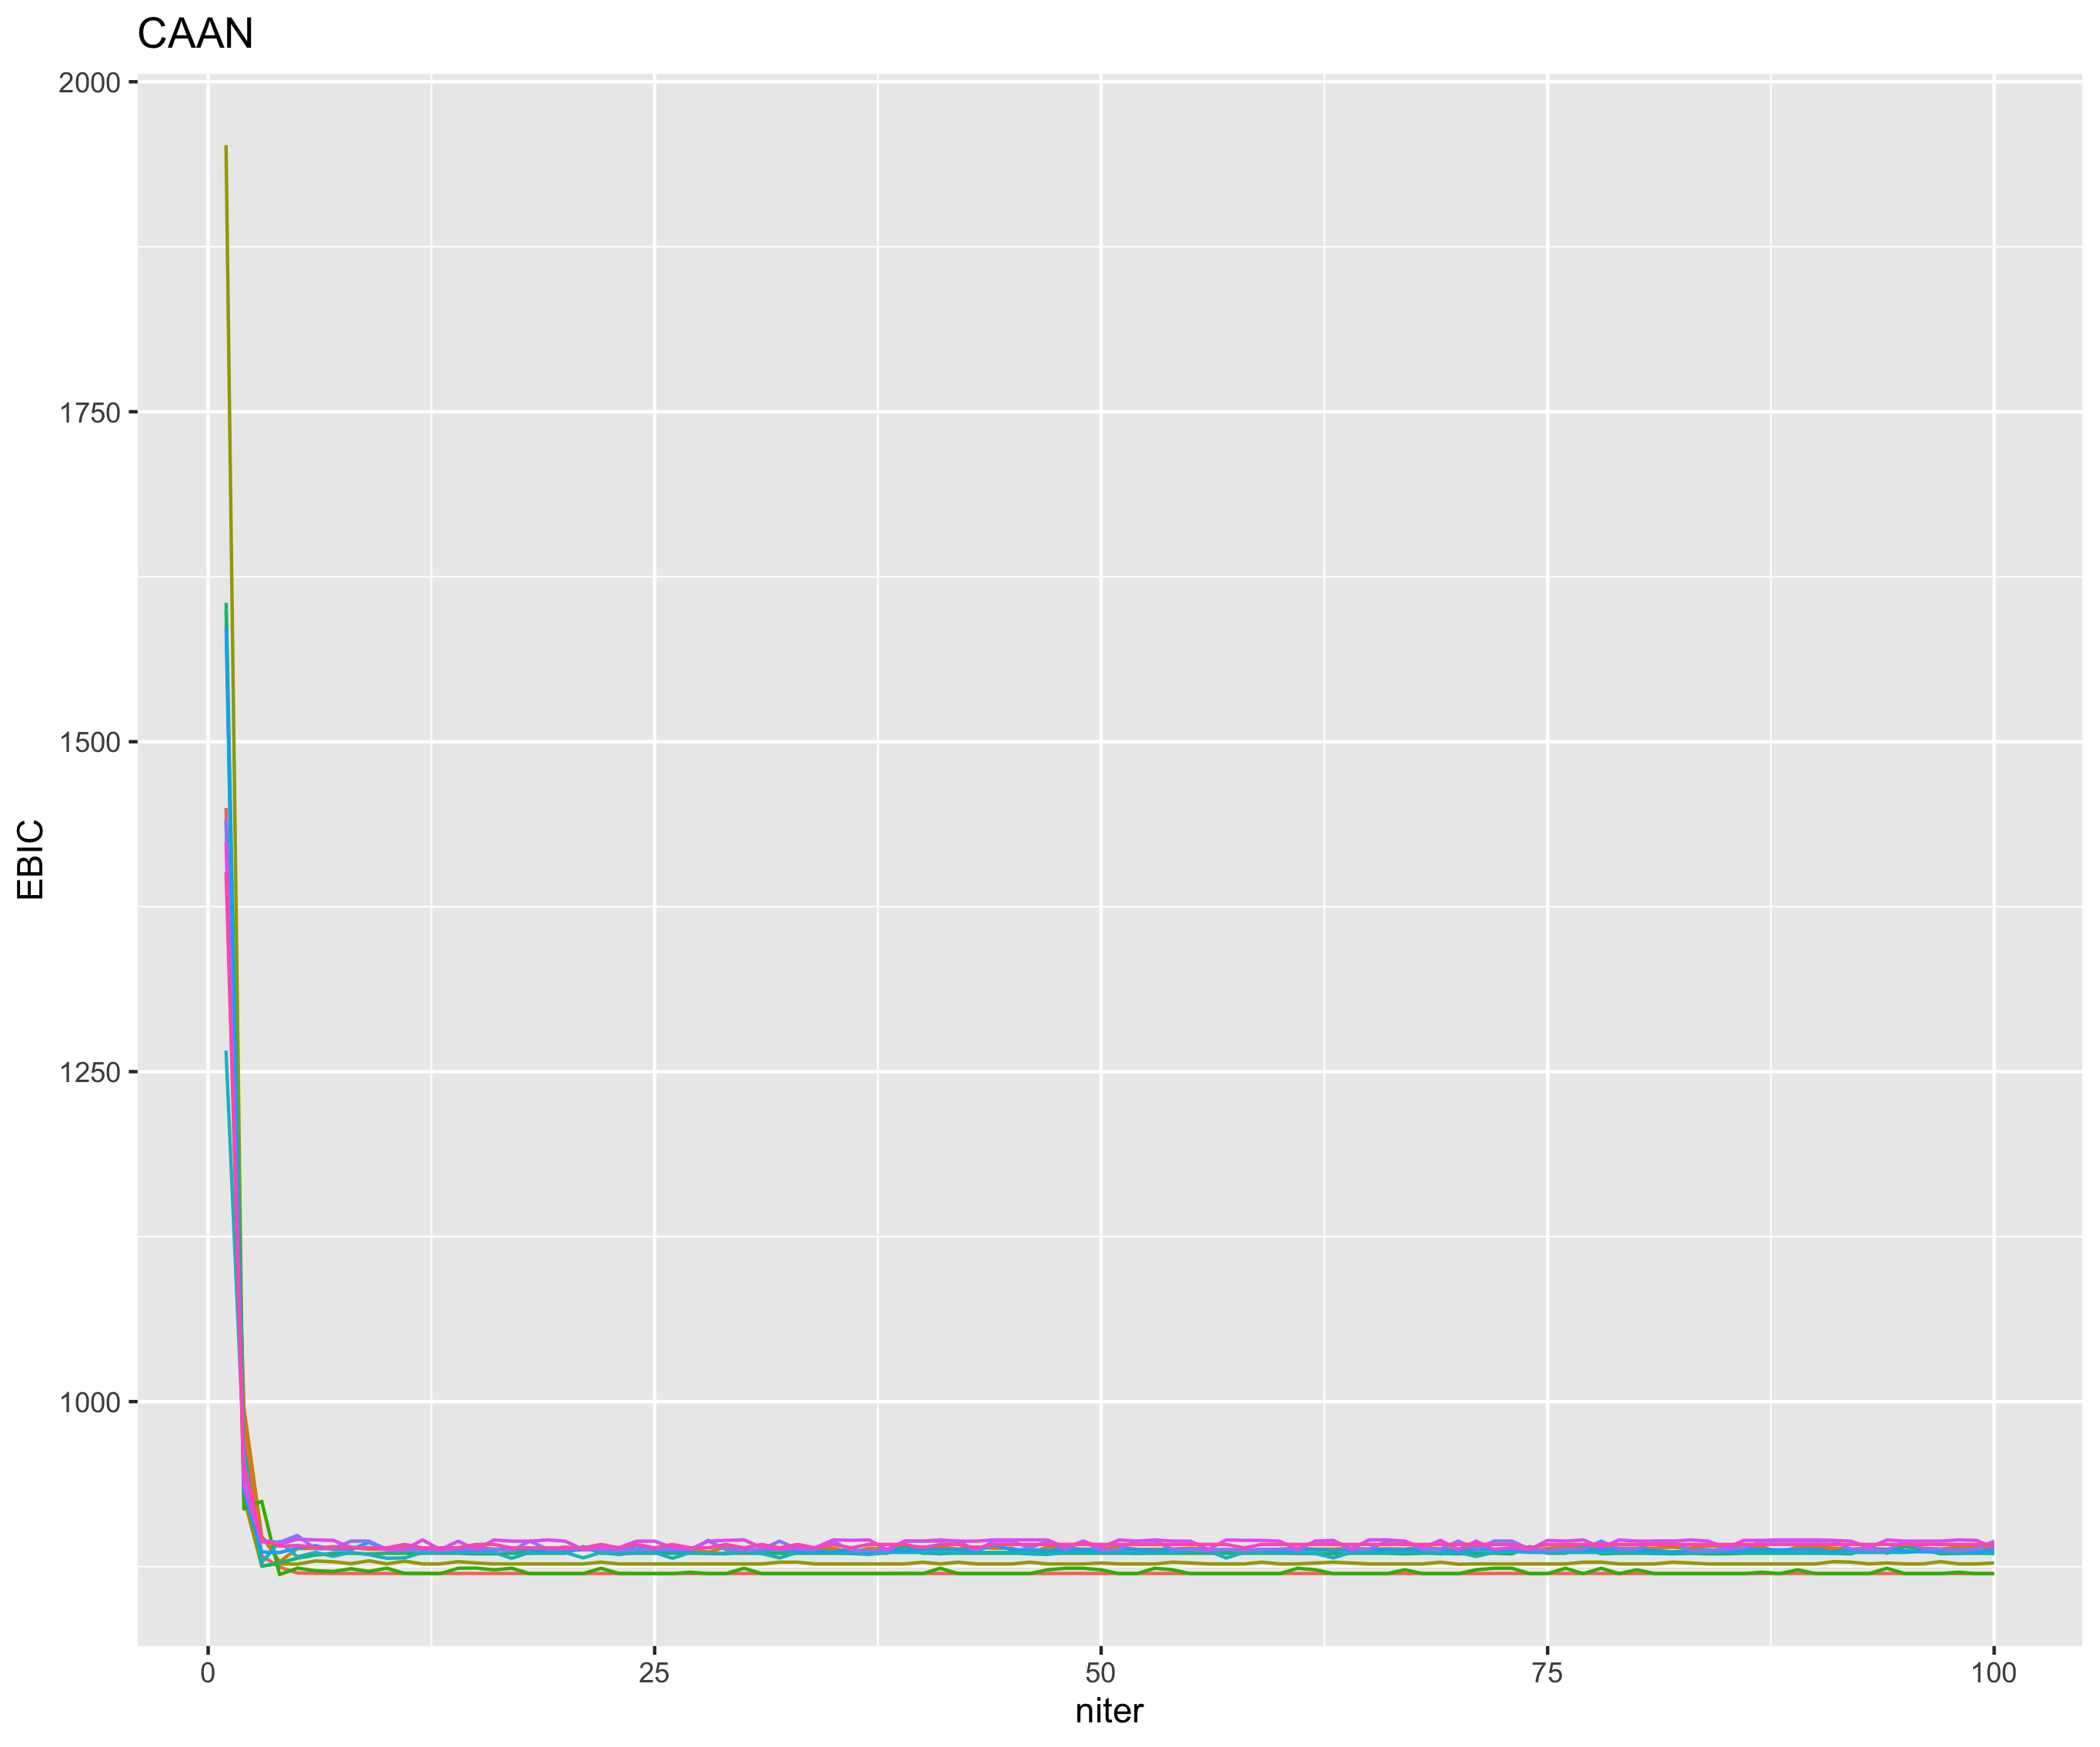
\includegraphics[width=\textwidth]{Figures/CAAN_EBIC.png}
     \end{subfigure}
        \caption{Trace plots of the log-MSE (top row) and EBIC (bottom row) paths from 10 different initial points for the EMVA and the CAAN optimization algorithms, based on a synthetic dataset generated (n = 120 and p = 200) with the true model 10. }
        \label{fig:Opt_comparison}
\end{figure}
